\lecture{1}{lun 01 mag 2023 16:51}{Intro}
	Iniziamo:
	\section{Definizioni}
	\begin{itemize}
		\item \textbf{Sistema}: la cosa che vogliamo controllare.
		\item \textbf{Controllo automatico}: senza o parziale controllo umano.
		\item \textbf{Controllo manuale}: azione esercitata dal l'operatore
	\end{itemize}
	\subsection{Notazione Standard}
	
	\begin{figure}[H]
		\begin{tikzpicture}[thick]
			\draw[->] (-9,0) -- (-8,0) node[above]{$ y^0 $} node[below,darkorange]{set point o riferimento}--(-7,0);
			\draw[rounded corners] (1,.5) rectangle (-1,-0.5); 
			\draw (0,0) node[scale=1.5]{S};
			\draw[->] (0,1.5) -- (0,1) node[above left]{d} -- (0,.5);
			\draw (0,1) node[above right,darkorange]{disturbo};
			\draw[->] (-3,0)node[below,darkorange]{variabile di controllo} --(-2,0)node[above]{u} -- (-1,0);
			\draw[<-] (3,0)node[below,darkorange]{variabile controllata} -- (2,0)node[above]{$ y $} -- (1,0);
			\draw (0,-.5) node[below,darkorange]{sistema};
		\end{tikzpicture}
		%		\centering
		%		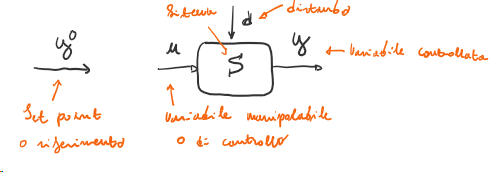
\includegraphics[width=0.7\linewidth]{Images/notazione_standard}
		%		\caption{rappresentazione generica di un sistema}
		%		\label{fig:notazionestandard}
	\end{figure}
	Notazioni:
	\begin{itemize}
		\item \textbf{Disturbo}: Tutto quello che non so o tutto quello che agisce esternamente
		\item \textbf{Set Point}: Risultato che voglio raggiungere
		\item \textbf{Variabile manipolabile}: Cosa faccio per modificare il sistema
		\item \textbf{Controllata}: Risultato, Objective $y = y^0$
		\item \textbf{Problema di controllo}: Assegnare ad $u$ un valore tale che $ y= y^0 $ 
		\item \textbf{Legge di controllo}: criterio scelto per generare $ u $
	\end{itemize}
	\subsection{Sistema ad anello}
	\begin{figure}[H]
		\centering
		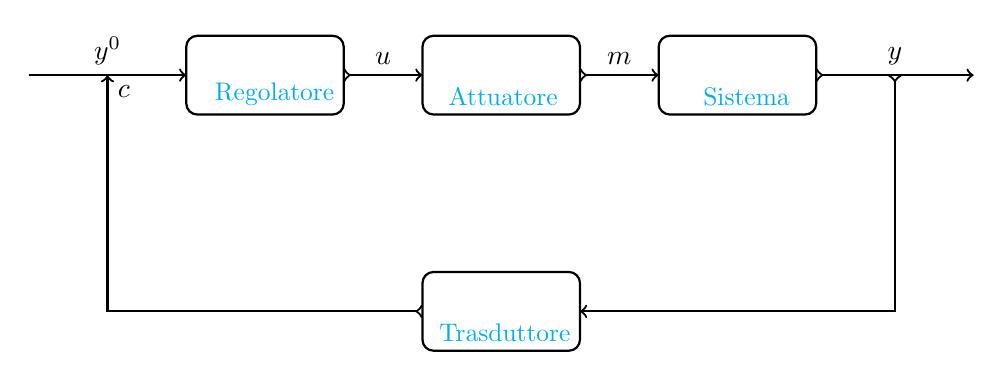
\begin{tikzpicture}[thick]
			\draw[->] (-5,0) -- (-4,0) node[above]{$ y^0 $} -- (-3,0);
			\draw[rounded corners] (-3,.5) rectangle (-1,-.5) node[above left, scale=0.92,cyan]{Regolatore};
			\draw[>->,xshift=3cm] (-4,0)--(-3.5,0) node[above]{$ u $} -- (-3,0);
			\draw[rounded corners,xshift=3cm] (-3,.5) rectangle (-1,-.5) node[above left, scale=0.92,cyan]{\, Attuatore \,};
			\draw[>->,xshift=6cm] (-4,0)--(-3.5,0) node[above]{$ m $} -- (-3,0);
			\draw[rounded corners,xshift=6cm] (-3,.5) rectangle (-1,-.5) node[above left, scale=0.92,cyan]{\,\, Sistema \,\,};
			\draw[>->,xshift=10cm] (-5,0)--(-4,0) node[above]{$ y $} -- (-3,0);
			\draw[>->] (6,0) -- (6,-3) -- (2,-3);
			\draw[rounded corners,xshift=3cm,yshift=-3cm] (-3,.5) rectangle (-1,-.5) node[above left, scale=0.92,cyan]{Trasduttore};
			\draw[<-<,rotate around y=180,xshift=2cm] (6,0)node[below right]{$ c $}  -- (6,-3) -- (2,-3);
		\end{tikzpicture}
		%		\includegraphics[width=0.7\linewidth]{"Images/Anello Chiuso"}
		\label{fig:anello-chiuso}
	\end{figure}
	
	Un sistema ad anello può essere suddiviso in due sotto-categorie: Anello \emph{Chiuso} e Anello \emph{Aperto}\\
	In figura è dato un sistema ad anello chiuso. In questo schema l'attuatore trasforma $ u $ in $ m $ (Esempio: voltaggio in energia meccanica $ \to $ Motore)

